\documentclass[12pt]{article}
\usepackage{microtype}

% The preceding line is only needed to identify funding in the first footnote. If that is unneeded, please comment it out.
\usepackage{amsmath,amssymb,amsfonts}
\usepackage{algorithmic}
\usepackage{graphicx}
\usepackage{textcomp}
\usepackage{xcolor}
\usepackage{url}
\usepackage{listings}
\usepackage{courier}
\usepackage{xspace}
\usepackage{multirow}
\usepackage{colortbl}
\usepackage{blindtext}
\usepackage{float}
\usepackage{hyperref}
%\usepackage[font=scriptsize]{caption}
%\newcommand{\sd}[1]{\textbf{"\textsc{SD:}} \textit{#1}"}
%Dessin
\usepackage{tikz}
\usepackage{verbatim}
\usepackage{graphicx}
\usepackage[utf8]{inputenc}
\usepackage[english]{babel}
\usepackage{subfigure}
 \newboolean{showcomments}
\setboolean{showcomments}{true}
\ifthenelse{\boolean{showcomments}}
  {\newcommand{\bnote}[2]{
	\fbox{\bfseries\sffamily\scriptsize#1}
    {\sf\small$\blacktriangleright$\textit{#2}$\blacktriangleleft$}
    % \marginpar{\fbox{\bfseries\sffamily#1}}
   }
   \newcommand{\cvsversion}{\emph{\scriptsize$-$Id: macros.tex,v 1.1.1.1 2007/02/28 13:43:36 bergel Exp $-$}}
  }
  {\newcommand{\bnote}[2]{}
   \newcommand{\cvsversion}{}
  } 


\newcommand{\here}{\bnote{***}{CONTINUE HERE}}
\newcommand{\nb}[1]{\bnote{NB}{#1}}

\newcommand{\fix}[1]{\bnote{FIX}{#1}}
%%%% add your own macros 


\newcommand{\an}[1]{\bnote{Anne}{#1}}
\newcommand{\sd}[1]{\bnote{Stef}{#1}}
\newcommand{\ja}[1]{\bnote{Jannik}{#1}}
\newcommand{\md}[1]{\bnote{MD}{#1}}
\newcommand{\caro}[1]{\bnote{Caro}{#1}}
\newcommand{\jr}[1]{\bnote{JRe}{#1}}
\newcommand{\lf}[1]{\bnote{Luc}{#1}}
\newcommand{\gp}[1]{\bnote{Guille}{#1}}
\newcommand{\pt}[1]{\bnote{Pablo}{#1}}
\newcommand{\theo}[1]{\bnote{Theo}{#1}}
\newcommand{\spb}[1]{\bnote{Santiago}{#1}}
\newcommand{\bv}[1]{\bnote{Beno\^{i}t}{#1}}

\graphicspath{{figures/}}
%%% 


\newcommand{\figref}[1]{Figure~\ref{fig:#1}}
\newcommand{\figlabel}[1]{\label{fig:#1}}
\newcommand{\tabref}[1]{Table~\ref{tab:#1}}
\newcommand{\layout}[1]{#1}
\newcommand{\commented}[1]{}
\newcommand{\secref}[1]{Section \ref{sec:#1}}
\newcommand{\seclabel}[1]{\label{sec:#1}}

%\newcommand{\ct}[1]{\textsf{#1}}
\newcommand{\stCode}[1]{\textsf{#1}}
\newcommand{\stMethod}[1]{\textsf{#1}}
\newcommand{\sep}{\texttt{>>}\xspace}
\newcommand{\stAssoc}{\texttt{->}\xspace}

\newcommand{\stBar}{$\mid$}
\newcommand{\stSelector}{$\gg$}
\newcommand{\ret}{\^{}}
\newcommand{\msup}{$>$}
%\newcommand{\ret}{$\uparrow$\xspace}

\newcommand{\myparagraph}[1]{\noindent\textbf{#1.}}
\newcommand{\eg}{\emph{e.g.,}\xspace}
\newcommand{\ie}{\emph{i.e.,}\xspace}
\newcommand{\etal}{\emph{et al.,}\xspace}
\newcommand{\ct}[1]{{\textsf{#1}}\xspace}


\newenvironment{code}
    {\begin{alltt}\sffamily}
    {\end{alltt}\normalsize}

\newcommand{\defaultScale}{0.55}
\newcommand{\pic}[3]{
   \begin{figure}[h]
   \begin{center}
   \includegraphics[scale=\defaultScale]{#1}
   \caption{#2}
   \label{#3}
   \end{center}
   \end{figure}
}

\newcommand{\twocolumnpic}[3]{
   \begin{figure*}[!ht]
   \begin{center}
   \includegraphics[scale=\defaultScale]{#1}
   \caption{#2}
   \label{#3}
   \end{center}
   \end{figure*}}

\newcommand{\infe}{$<$}
\newcommand{\supe}{$\rightarrow$\xspace}
\newcommand{\di}{$\gg$\xspace}
\newcommand{\adhoc}{\textit{ad-hoc}\xspace}

\usepackage{url}            
\makeatletter
\def\url@leostyle{%
  \@ifundefined{selectfont}{\def\UrlFont{\sf}}{\def\UrlFont{\small\sffamily}}}
\makeatother
% Now actually use the newly defined style.
\urlstyle{leo}




 
\author{
        Bragagnolo, Santiago
}
\title{TP GIS4 - Anti-monopoly}
\date{\today}

 
\begin{document}
\maketitle
\emph{Cet exercise est basé sur un exercice proposé dans le cour de Paradigmes de programmation, à l'UTN, Argentine.}

\section{Introduction}

\begin{figure}
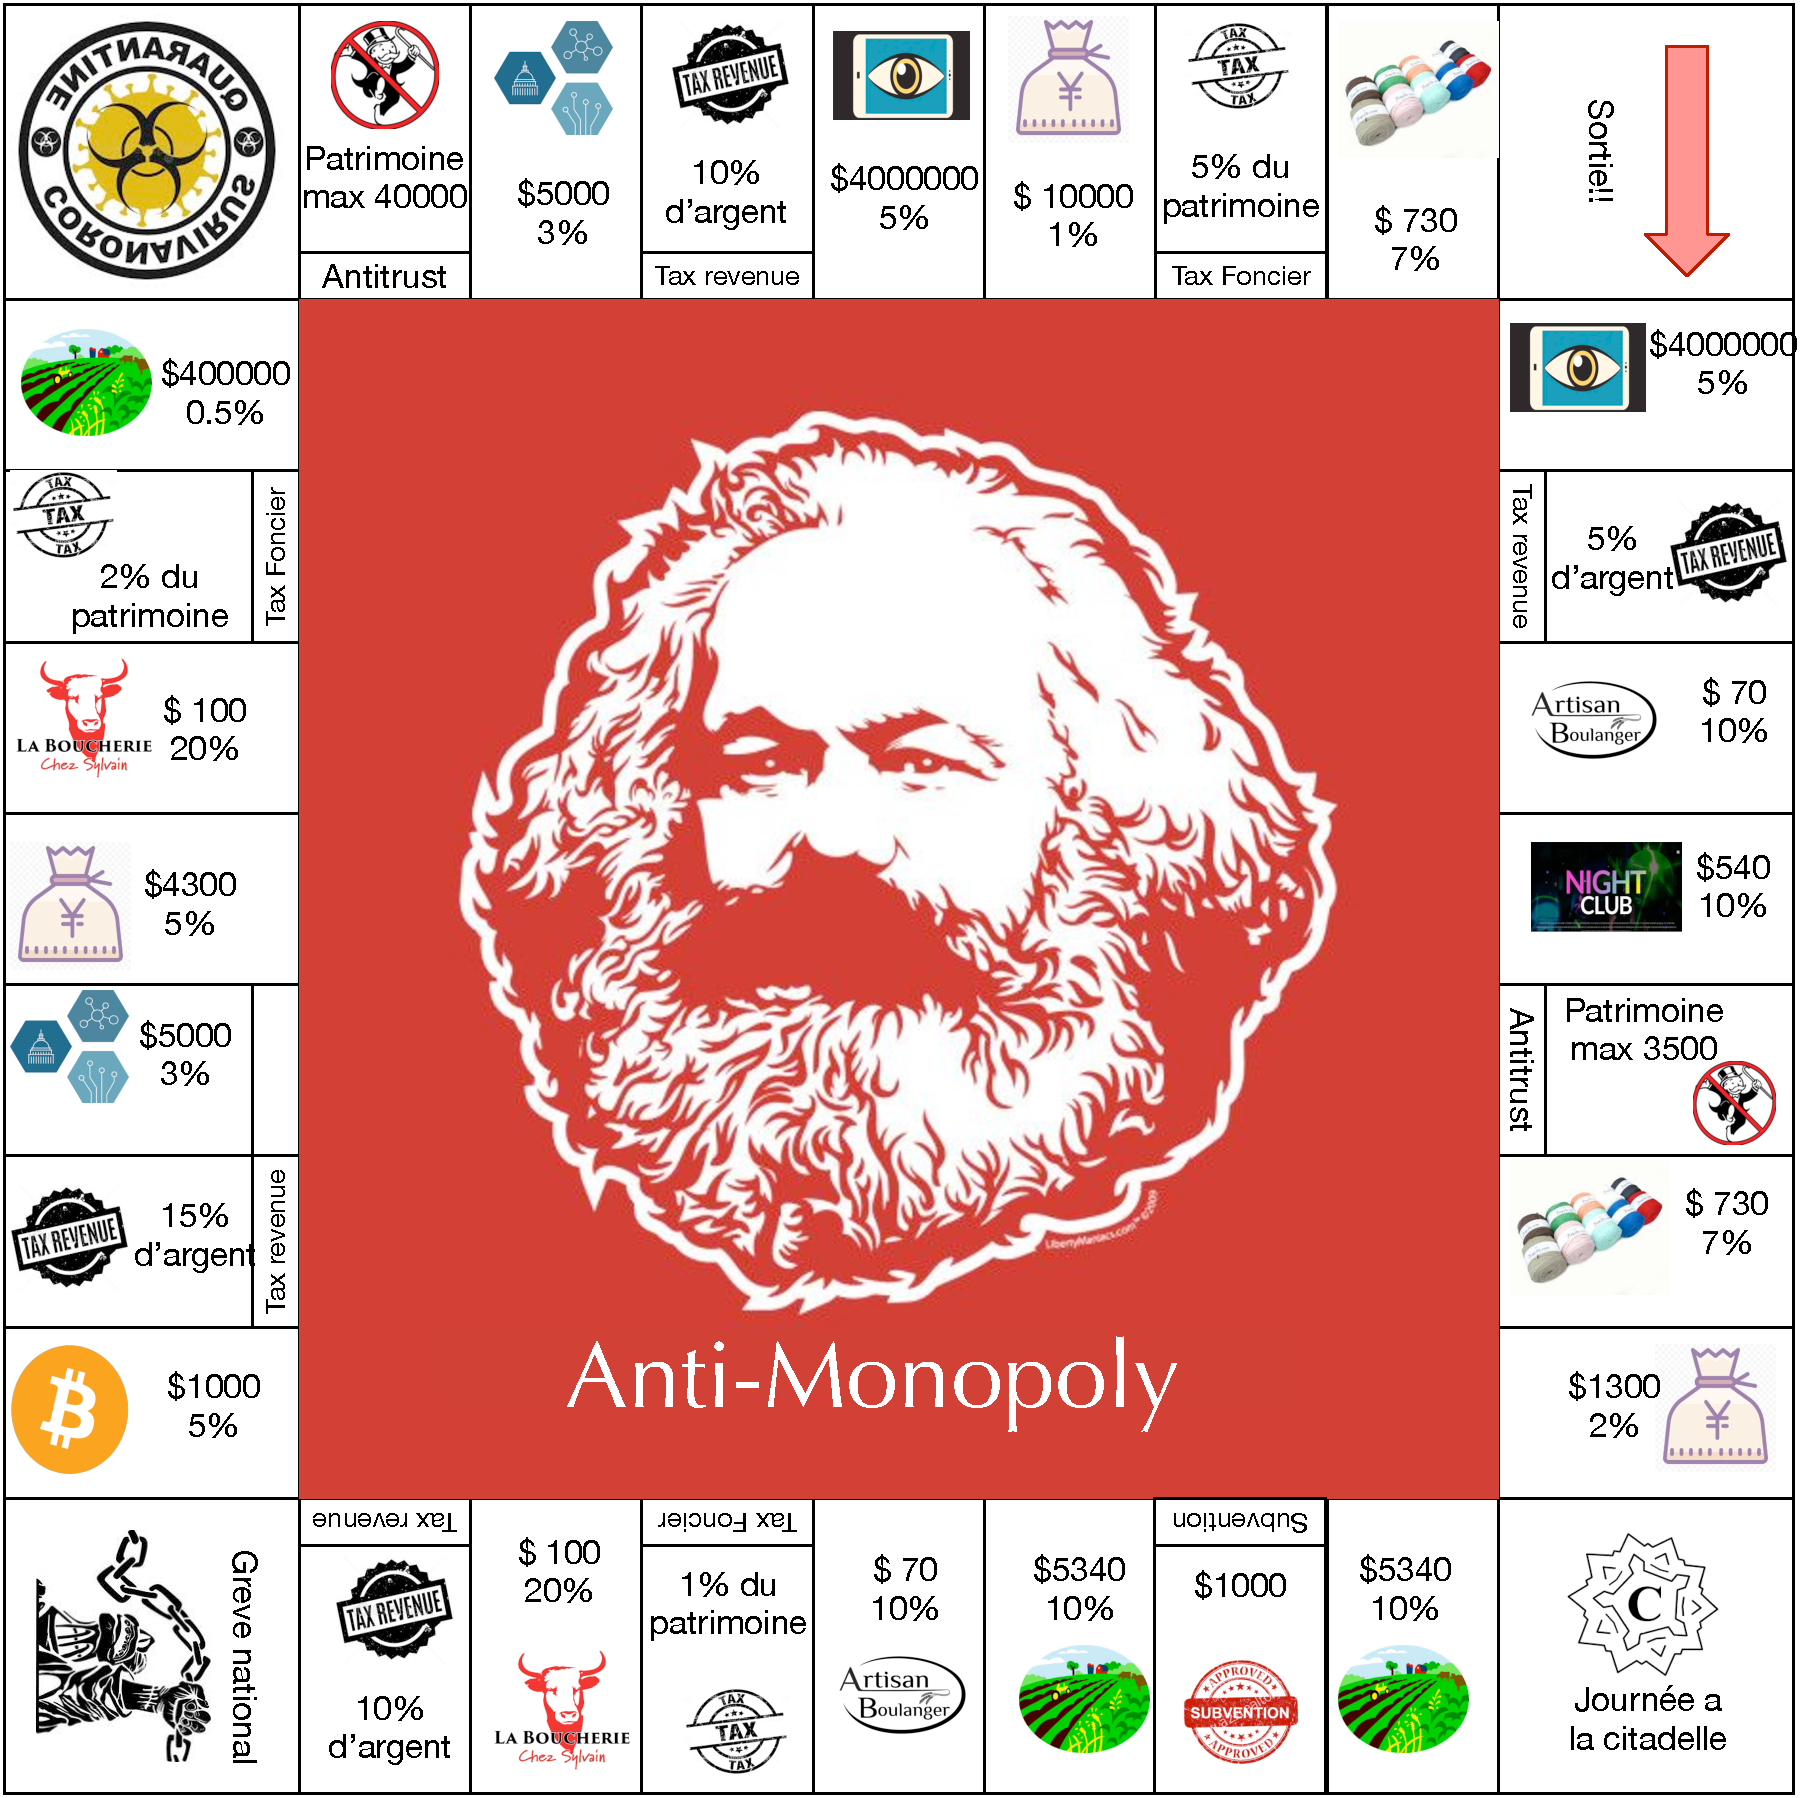
\includegraphics[width=15cm,height=15cm,keepaspectratio]{figures/board.pdf}
\caption{Exemple de tableau de jeu}
\end{figure}



	Vous souhaitez implémenter un jeu du style \emph{Monopoly} dans lequel les joueurs cherchent
à augmenter leur patrimoine en marchant sur un chemin où ils doivent prendre des décisions 
d'investissement et faire certaines actions. Attention toutefois à ne pas trop investir, car 
les lois antitrust peuvent vous obliger à distribuer votre richesse.


\section{Caractéristiques du jeu}

    \subsection{Plateau du jeu}
    Le \textbf{plateau} est constitué d'un chemin circulaire composé de \textbf{cases},
dans chacune desquelles il y a des indications. Une case marquée \textbf{sortie}
indique le point de départ du jeu.

    \subsection{Joueurs}
    Il peut y avoir autant de \textbf{joueurs} que souhaité. Chaque joueur a un
montant d'argent initial. Au fur et à mesure que le jeu progresse, chacun des joueurs accroit
ou décroit son argent, selon les décisions d'investissement qu'ils prennent ou d'autres
circonstances. Les capitaux propres d'un joueur correspondent à
son argent plus l'évaluation de tous les investissements qu'il possède.
Si un joueur perd tous ses capitaux il a perdu: il ne peut pas continuer à jouer.
    
    \subsection{L'\'Etat}
    L'\'Etat est un acteur social dont la fonction principale est de réguler l'activité économique des
différents joueurs. Il a des ressources financières. L'État ne participe pas
au jeu en marchant sur le plateau, mais interagit avec tous les joueurs de différentes manières.

    \subsection{La dynamique de jeu}
    Initialement, tous les joueurs sont placés dans la case \textbf{sortie}. À tour de rôle, chacun lance
un \textbf{dé} et avance d'où il se trouve d'autant de cases que l'indique le
dé. Là, le joueur doit suivre les instructions
indiquées dans la case et prend les décisions économiques qu'il juge appropriées.
De cette façon, tous les joueurs avancent à travers le plateau et font leur
entreprise. Comme l'itinéraire est circulaire, il n'y a pas de point d'arrivée prédéterminé,
raison pour laquelle ils continuent à tourner jusqu'à ce que l'on souhaite mettre fin au jeu. \cfd{Préciser si un seul joueur peut décider d'y mettre fin ou si tous les joueurs doivent être d'accord.}
Le jeu est également terminé s'il ne reste qu'un seul joueur ou si l'État échoue.
    
    \subsection{Case}
        Il existe dans ce jeu différent type de cases. Voici leur particularités:
    \begin{itemize}
        \item \textbf{Investissement}: Si l'investissement est déjà possédé par un autre joueur, vous devez lui payer une somme d'argent proportion de la valeur de l'investissement.\an{pas compris cette phrase}\spb{TEXTE MODIFIE}\cfd{J'ai remodifié pour le rendre plus clair}.
        Si l'investissement est disponible, le joueur décide s'il veut le prendre ou le laissez passer. 
	
        \item \textbf{Loi antitrust}: Oblige le joueur à céder tous les investissements
    qu'il possède et qui dépassent le maximum fixé par l'État. 
    Ces investissements reviennent à l'Etat, qui paie le joueur la moitié de leur prix. 
    Une fois entre les mains de l'état, ces investissements deviennent de nouveau disponibles si un joueur rentre dans cette case. 
    \an{ca veut dire quoi qu'il reste a nouveau dispo}.\spb{TEXTE MODIFIE}\cfd{J'ai remodifié pour le rendre plus clair}
        \item  \textbf{Bureau Finances publiques}: Oblige le joueur à payer à l'État un pourcentage de ses
    capitaux propres, au cas où ils dépasseraient une certaine valeur. Chaque taxe se calcule comme un pourcentage du patrimoine du joueur.
    Le pourcentage de chaque type d'impôt (impôt sur le revenu, impôt foncier personnel, etc.) est différent. \an{pas compris la dernière phrase}\spb{TEXTE MODIFIE}\cfd{J'ai remodifié pour le rendre plus clair}
        \item \textbf{Subvention}: Le joueur reçoit de l'État le montant indiqué dans la case.
        \item \textbf{Repos}: C'est une case vide dans laquelle rien ne se passe. La \textbf{sortie} en fait partie.
    \end{itemize}
    
    \begin{figure}
    \centering
    \subfigure[]{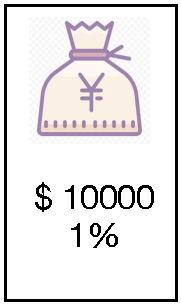
\includegraphics[width=2cm,height=2cm,keepaspectratio]{figures/investissement.pdf}} 
    \subfigure[]{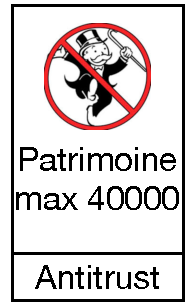
\includegraphics[width=2cm,height=2cm,keepaspectratio]{figures/antitrust.pdf}} 
    \subfigure[]{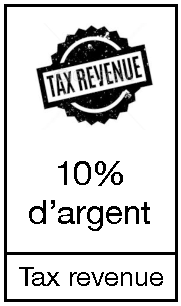
\includegraphics[width=2cm,height=2cm,keepaspectratio]{figures/taxe.pdf}}
    \cfd{Il manque la subvention}
      \subfigure[]{
\includegraphics[width=2cm,height=2cm,keepaspectratio]{figures/rienfaire.pdf}}

   
    \caption{(a) Investissment (b) Loi antitrust (c) Finances publiques (d) Subvention (e) Activite non comercial}
    \label{fig:foobar}
\end{figure}



    \subsection{Investissements}
	Les \textbf{investissements} sont le principal moyen pour les joueurs de gagner de l'argent. Initialement
l'\'Etat possède tous les investissements. Ils ont chacun un prix de référence, correspondant au
montant à payer par le joueur lorsqu'il tombe dans la case correspondant à celui-ci et décide de l'assumer.
Chaque investissement génère un revenu calculé en pourcentage du prix de
référence, qui est chargé au joueur qui tombe dans la case \spb{TEXTE MODIFIE}\an{pas compris}\cfd{Ce n'est pas clair. Je n'ai pas compris si le pourcentage à payer est sur le capital du joueur ou sur le prix de l'investissement}. 
Le prix et pourcentages de les bénéfices d'investissement sont arbitraires.

    \subsection{Style des joueurs}
    Le fait qu'un joueur accepte ou non de conserver un investissement dépend en premier lieu 
    de s'il a assez d'argent, mais aussi d'un style de jeu. associé à ce joueur. 
    Il existe différents styles de jeu qui sont les suivants :
        \begin{itemize}
           \item \textbf{Prudent}: Le joueur accepte l'investissement que s'il a moins d'un certain montant 
           d'investissements et que la valeur du nouvel investissement représente moins de 20 \% de ses
           actifs actuels.
           \item  \textbf{Agressif}: Le joueur achète tout.
        \end{itemize}

    Finalement, si un joueur est obligé de se séparer de certains investissements, 
    il les choisit en fonction de son style de jeu:
        \begin{itemize}
            \item \textbf{Prudent}: Il choisit en priorité le plus cher.
            \item \textbf{Agressif}: Il choisit en priorité le moins cher.
        \end{itemize}
        
\section{Exigences du projet}
Sur la base de l'approche générale du jeu, l'implémentation demandée doit comprendre :

\subsection{Définition initiale}
Créez un plateau de jeu avec plusieurs cases (au moins 10), des joueurs (au moins 2, un de
chaque style de jeu) et l'État. Il faut définir les prix, pourcentages, capitaux et valeurs initiales nécessaires. 
Il faut distribuer les quantités et valeurs des cases d'une manière que vous considérez comme équilibrée.

\subsection{Simulation}
 Dans le \texttt{main}, effectuez les étapes suivantes, en choisissant arbitrairement la valeur des dés:
 \begin{itemize}
\item   Localisez tous les joueurs à la sortie.
\item    Demander à un joueur d'avancer un certain nombre de cases et de faire l'action correspondante.
\item    Vérifier la situation financière du joueur.
\item    Faites jouer tous les joueurs en terminant un tour.
\item    Obtenez le classement des actifs des joueurs.
\item Simulez quelques tours jusqu'à ce qu'il ne reste qu'un joueur.
\end{itemize}


\subsection{Variantes} \cfd{À préciser si c'est requis ou si c'est du bonus}
Redémarrez le jeu en inventant les conditions initiales selon différentes
"Positions idéologiques", et voyez leur impact sur la simulation du jeu. Par
exemple :
\begin{itemize}
  \item \textbf{NeoLiberal}~: Certains joueurs avec beaucoup d'argent et d'autres avec peu, un état avec quelques
mesures antitrust légères.
  \item \textbf{Socialiste}~: Tous les joueurs avec le même argent de départ, beaucoup de taxes.
  \item \textbf{Capitaliste}~: tous les joueurs agressifs, pourcentages de profit élevés, plus élevés
ratio d'investissement.
  \item \textbf{Progressiste} : plus de joueurs, des lois antitrust strictes
combiné avec des subventions, des pourcentages de profit modérés.
  \item \textbf{l'Europe après le Covid-19} : (au choix de chacun).
\end{itemize}
\end{document}

